\documentclass[13pt]{beamer}				\usepackage{graphicx}
\usepackage{comment}
\usepackage{pdfpages}	
\usepackage{tikz}
\usepackage{comment}
\usepackage{relsize}
\usepackage{mathtools}
\usepackage{biblatex}
\addbibresource{biblio.bib}

\newcommand\Ccancel[2][black]{\renewcommand\CancelColor{\color{#1}}\xcancel{#2}}
\mode<presentation>						% Set options
{
  \usetheme{Madrid}					% Set theme
  \usecolortheme{seahorse} 				% Set colors
  \usefonttheme{default}  				% Set font theme
  \setbeamertemplate{caption}[numbered]	% Set caption to be numbered
}
\usepackage[makeroom]{cancel}
\definecolor{blue}{RGB}{88, 88, 191}
\definecolor{white}{RGB}{255, 255, 255}
\definecolor{uuuuuu}{rgb}{0.2666,0.2666,0.2666}
\definecolor{wwwwww}{rgb}{0.4,0.4,0.4}
\definecolor{ccqqqq}{rgb}{0.8,0,0}
\definecolor{qqqqff}{rgb}{0,0,1}


\usepackage{hyperref}					% For cross-referencing

\title[On the Information Bottleneck Theory]{On the Information Bottleneck Theory of Deep Learning}
\author[Polina Barabanshchikova]{Polina Barabanshchikova}	
\institute[MIPT]{MIPT}
\DeclareMathOperator{\rank}{rank}
\DeclareMathOperator{\dist}{dist}
\DeclareMathOperator{\conv}{conv}
\DeclareMathOperator{\tr}{tr}
\DeclareMathOperator{\degree}{deg}
\DeclareMathOperator{\cl}{cl}
\DeclareMathOperator{\argmin}{argmin}
\DeclareMathOperator{\lo}{\longleftrightarrow}
\DeclareMathOperator{\Lo}{\Longleftrightarrow}
\newcommand{\D}{\overline{D}}
\begin{document}

\begin{frame}
  \titlepage
\end{frame}

\begin{frame}{Motivation}
\textbf{Trajectory in the information plane}
is the amount of information in a hidden layer regarding the input and output measured over the
course of learning
\begin{figure}[h!]
    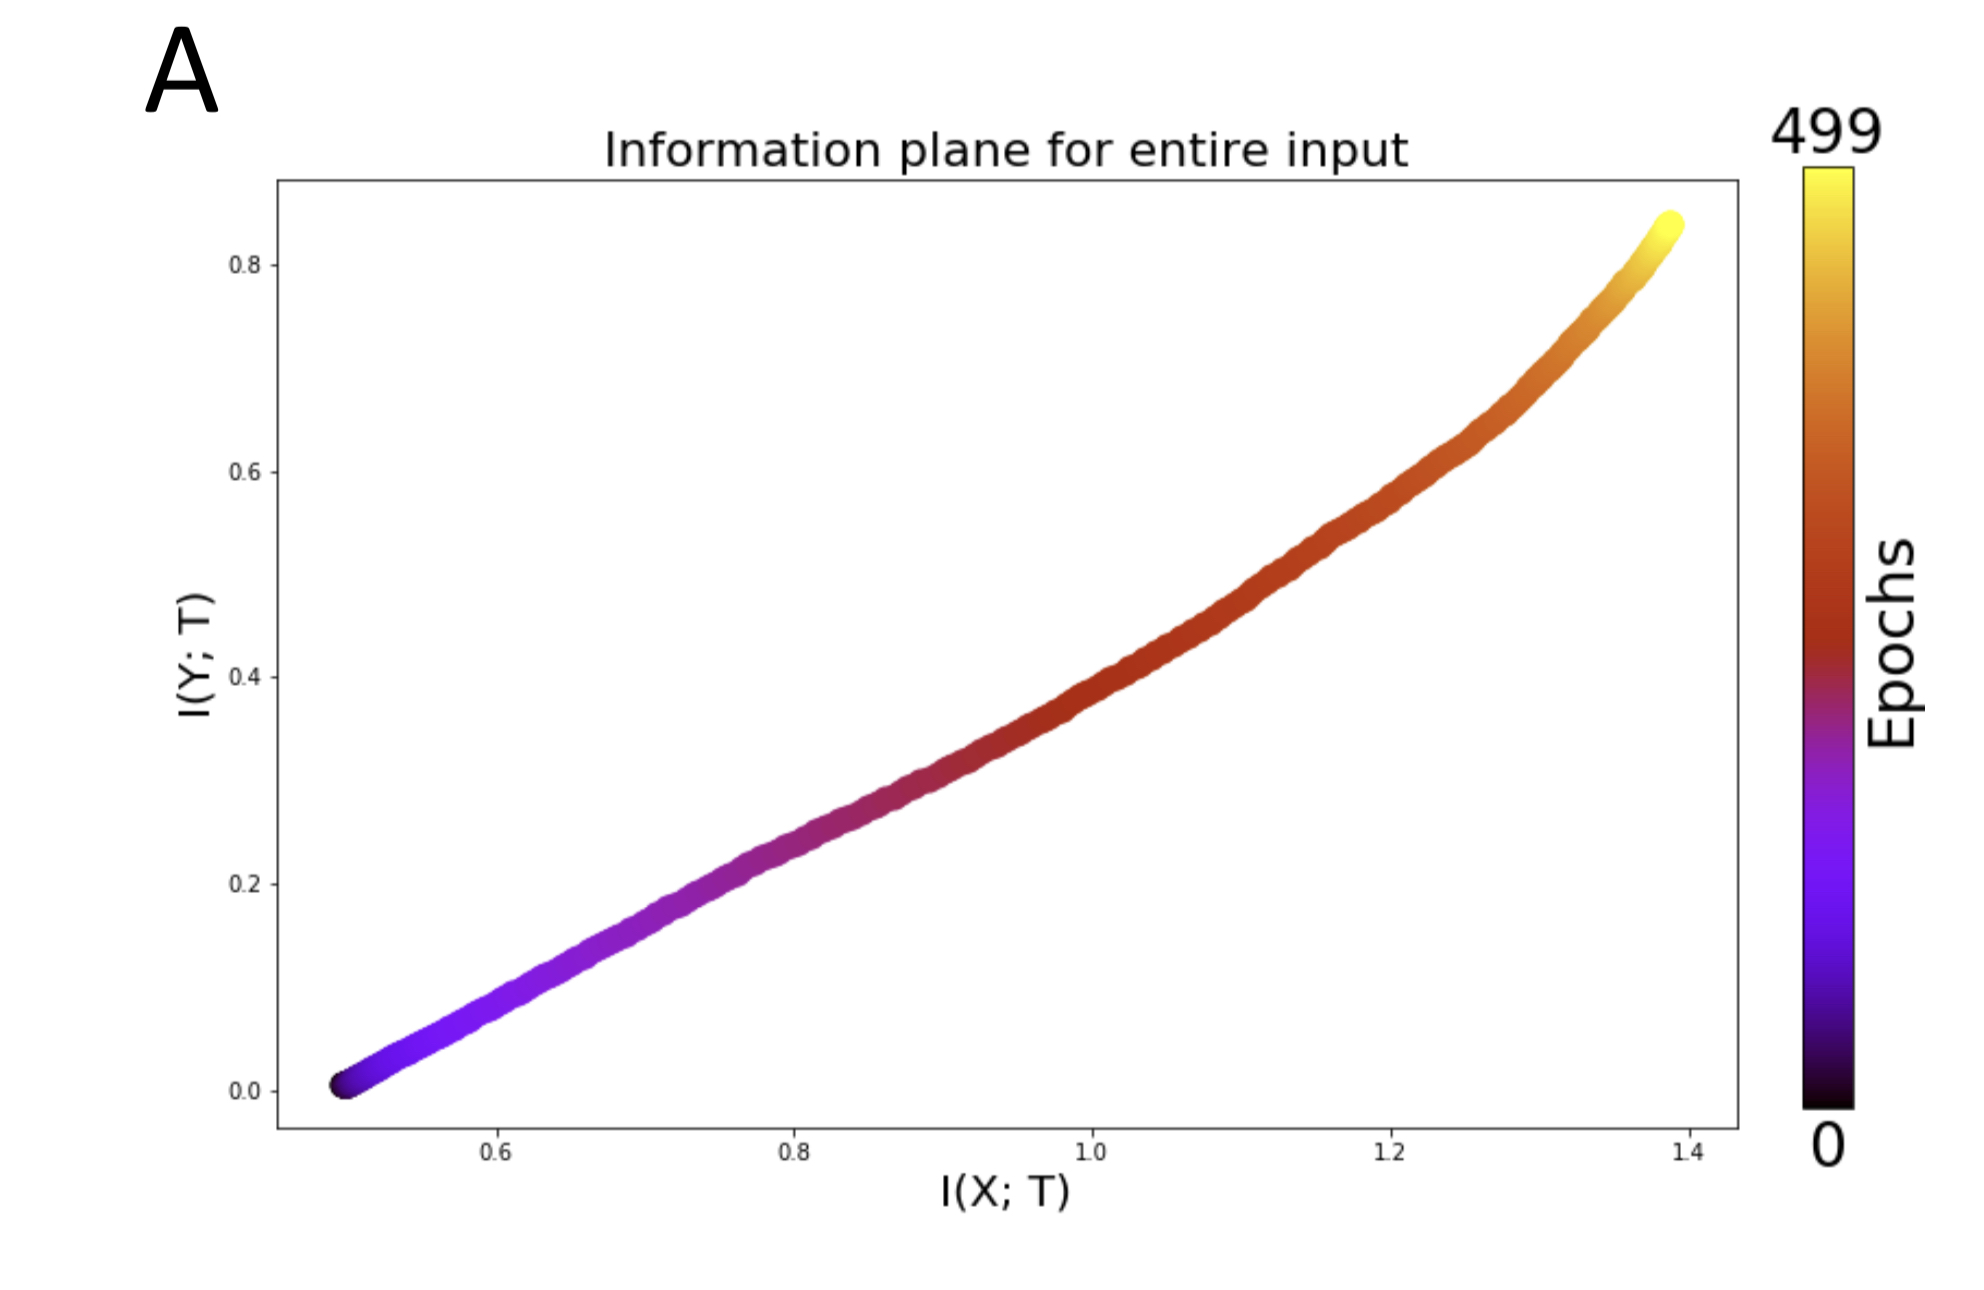
\includegraphics[width=0.7\textwidth, trim={0 0 0 0cm},clip]{images/InfB0.jpg}
\end{figure}
\end{frame}

\begin{frame}{Motivation}
\textbf{Observation}(Shwartz-Ziv, Tishby)

Trajectories in the information plane
consist of two distinct phases: 
\begin{itemize}
\item a “fitting” phase where mutual information between the hidden layers and both the input and output increases
\item a subsequent “compression” phase where mutual
information between the hidden layers and the input decreases
\end{itemize}
\textbf{Hypothesis}(Shwartz-Ziv, Tishby)
\begin{itemize}
\item compression phase is responsible for the excellent generalization performance
\item compression phase occurs due to the random diffusion-like behavior of stochastic
gradient descent
\end{itemize}
\end{frame}

\begin{frame}{Motivation}
\textbf{Fitting and compression phases}
\begin{figure}[h!]
    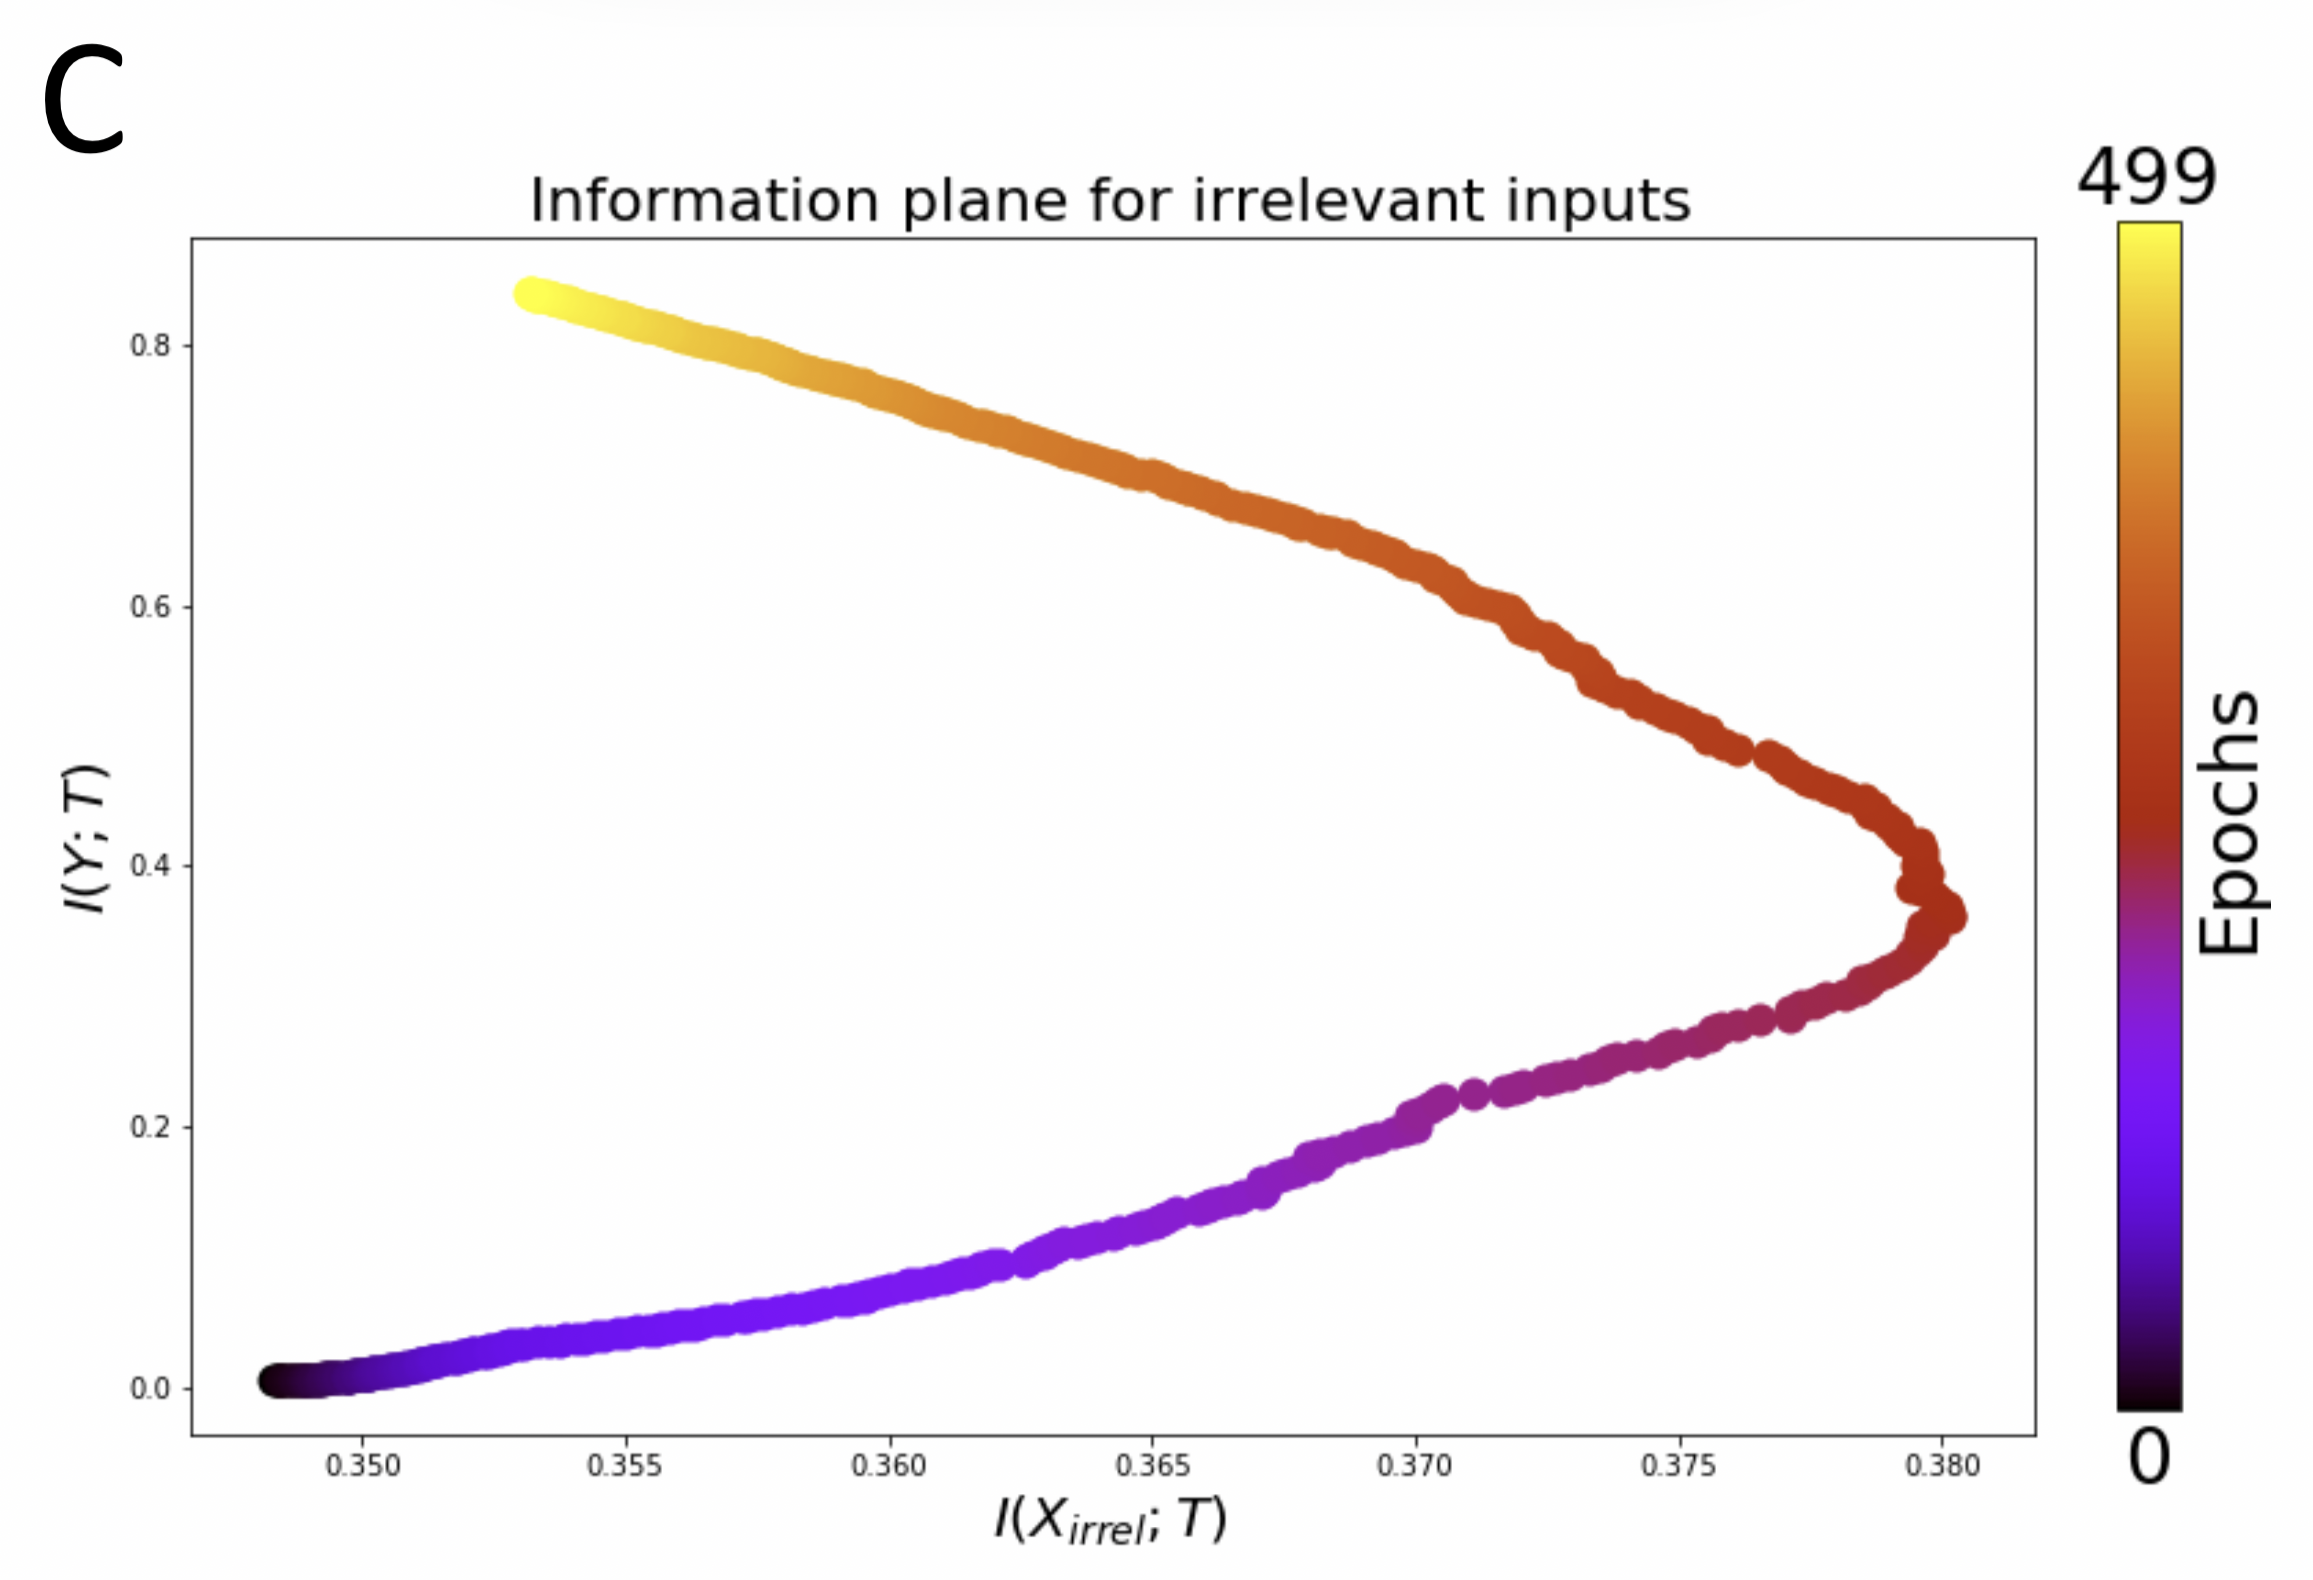
\includegraphics[width=0.7\textwidth, trim={0 0 0 0cm},clip]{images/InfB.PNG}
\end{figure}
\end{frame}

\begin{frame}{Results}
\begin{itemize}
    \item The information plane trajectory predominantly depends on the neural nonlinearity employed: double-sided saturating nonlinearities yield a compression phase, but others do not 
    \item There is no evident causal connection between compression and generalization
    \item The compression phase, when it exists, does not arise from stochasticity in training
\end{itemize}
\end{frame}

\begin{frame}{Method description. Minimal model}
Consider the simple three neuron
network with first layer weight $w_1$ and a nonlinearity $f$. Input $X \sim \mathcal{N}(0, 1)$ is fed through the net, yielding
the hidden unit activity $h = f (w_1 X)$. 

To calculate the mutual information with the input, this hidden unit activity is binned $T = \text{bin}(h)$ (into evenly spaced bins: from -1 to 1 for tanh and between the minimum and maximum activity values for relu).
$$I(T ; X) = H(T) - H(T | X) = H(T) = -\sum\limits_{i=1}^{N} p_i \log p_i,$$
where $p_i = P(h > b_i \text{ and } h < b_{i + 1})$.

The actual $I(h; X)$ is infinite.
\end{frame}

\begin{frame}{Experiments. Minimal model}
\begin{figure}[h!]
    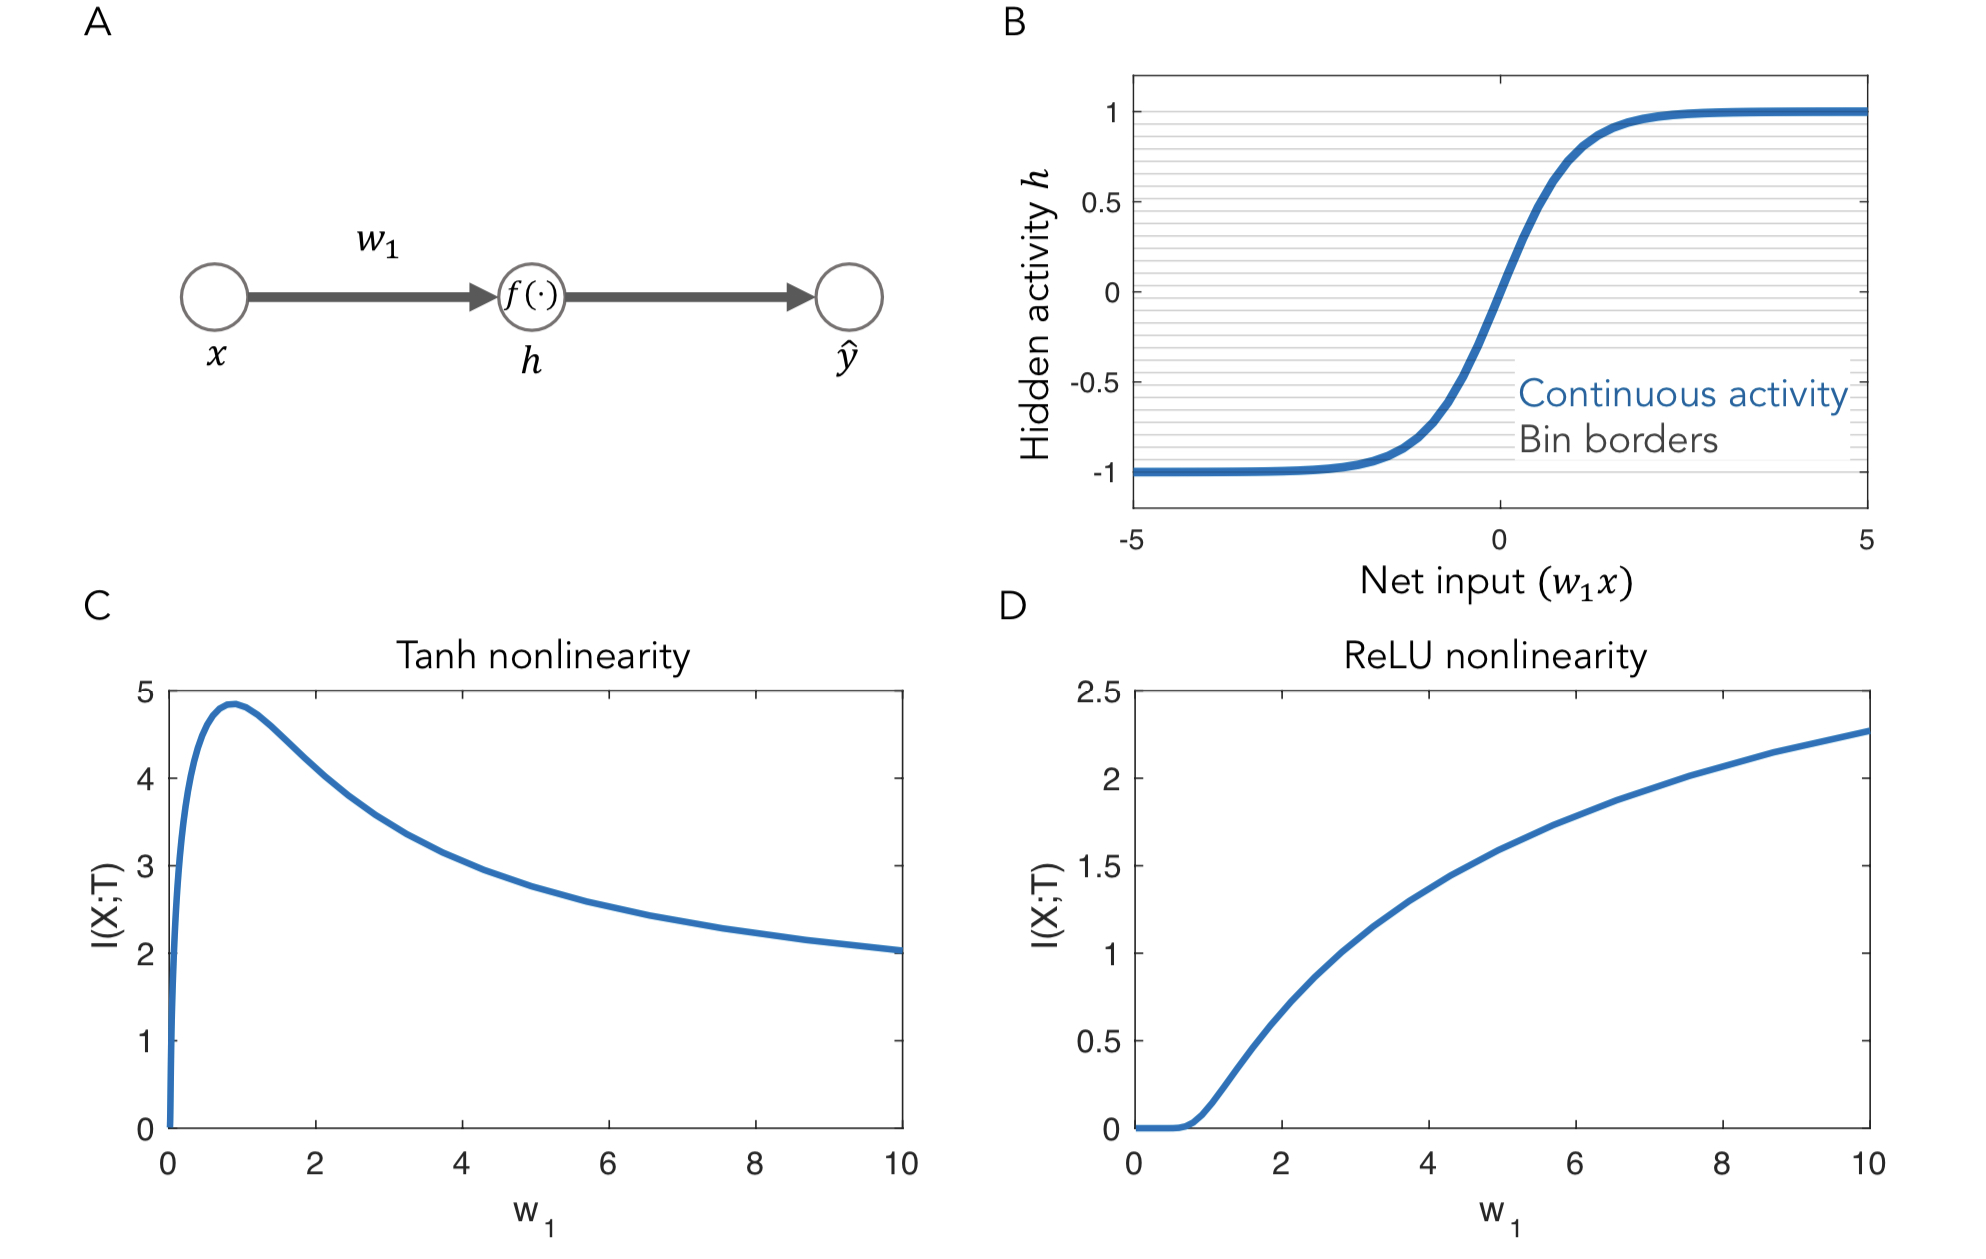
\includegraphics[width=1\textwidth, trim={0 0 0 0cm},clip]{images/InfB1.jpg}
\end{figure}
\end{frame}

\begin{frame}{Experiments. MLP}
\begin{figure}[h!]
    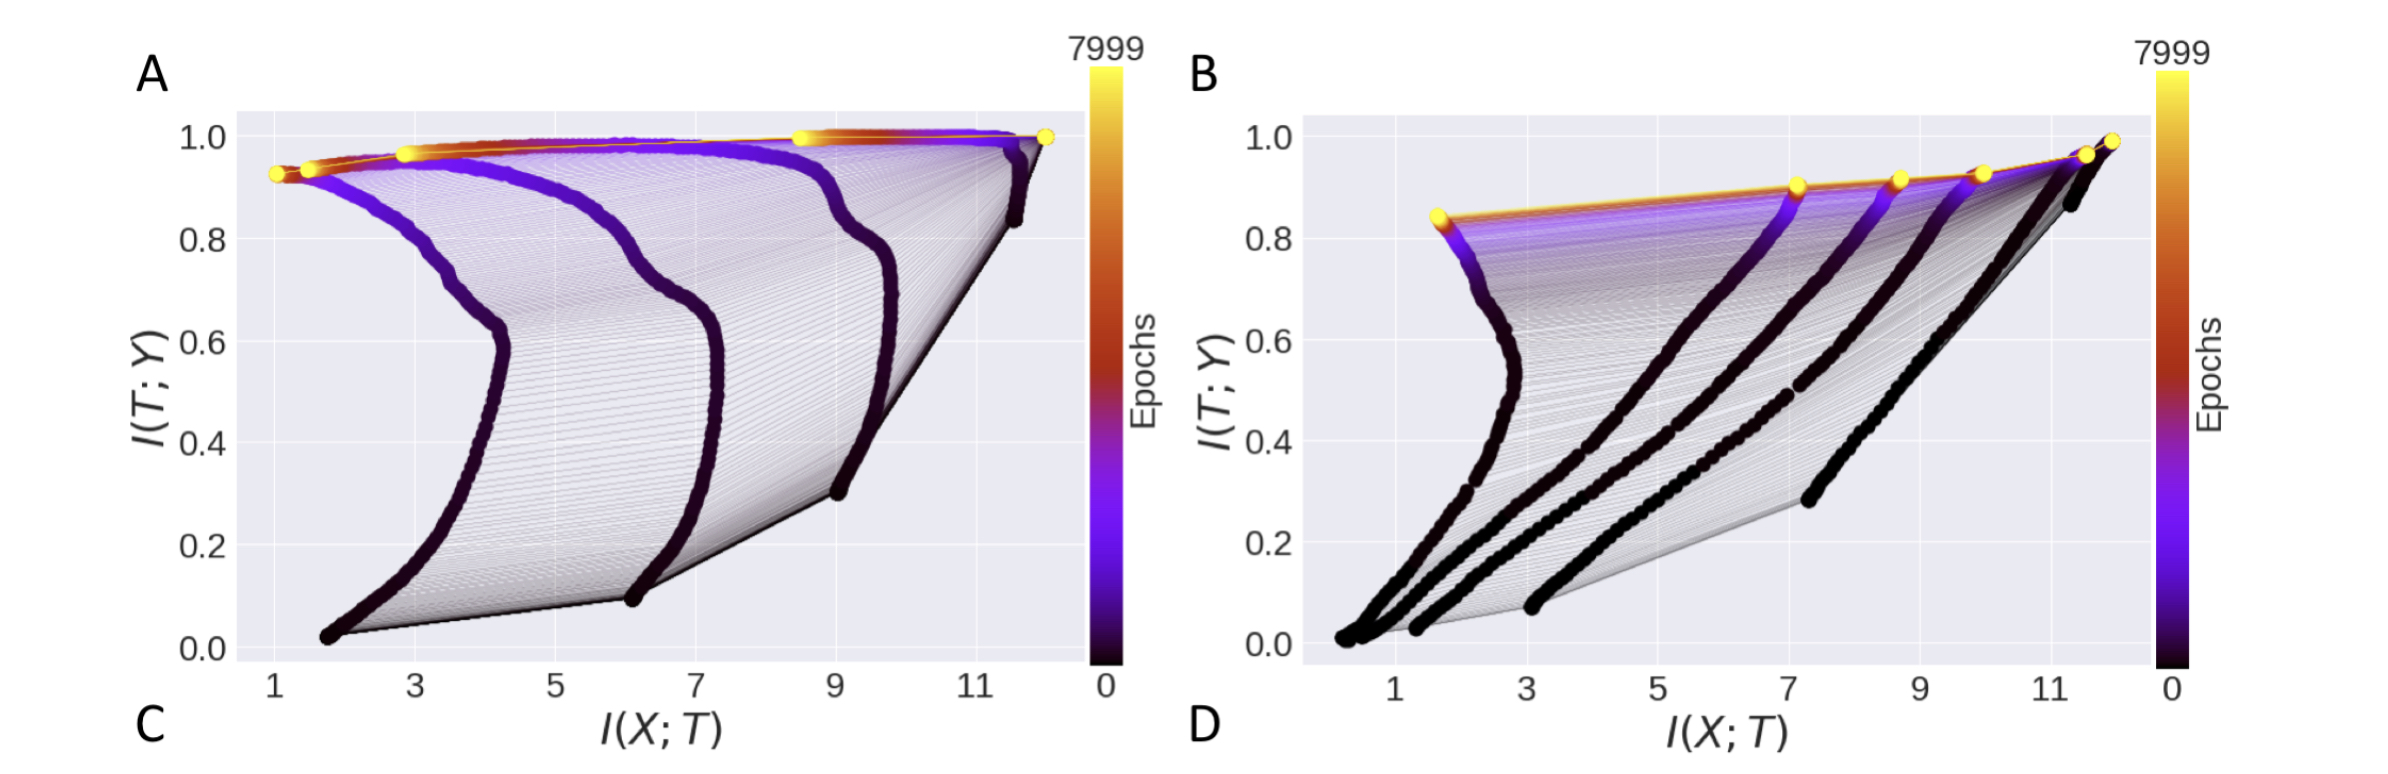
\includegraphics[width=1\textwidth, trim={0 0 0 0cm},clip]{images/InfB2.jpg}
    \caption{Information plane dynamics and neural nonlinearities. (A) Replication of Shwartz-Ziv and Tishby for a network with tanh nonlinearities. The x-axis plots information between each layer and the input,
while the y-axis plots information between each layer and the output. The color scale indicates
training time in epochs. Each of the six layers produces a curve in the information plane with the
input layer at far right, output layer at the far left. Different layers at the same epoch are connected
by fine lines. (B) Information plane dynamics with ReLU nonlinearities (except for the final layer
of 2 sigmoidal neurons).}
\end{figure}
\end{frame}

\begin{frame}{Method description. Generalization}
Consider a scenario where a linear teacher network generates input and output examples
which are then fed to a deep linear student network to learn. 

Assume $X \sim \mathcal{N}(0, 1)$ and $Y = W_0 X + \varepsilon_0$, where $\varepsilon_0 \sim \mathcal{N}(0, \sigma^2_0)$ and the weights $W_0$ are drawn independently from $\mathcal{N}(0, \sigma^2_w)$. 

The student network is trained to minimize the mean squared error between its output and the target. Here the student is a deep linear neural network consisting of potentially many layers, but without nonlinearities, that is $\hat{Y} = W_{D + 1} \dots W_1 X = W_{tot} X$.

For the purpose of calculating the mutual information, assume that Gaussian noise is added to the hidden layer activity, $T = W_{tot} X + \varepsilon$.
\end{frame}

\begin{frame}{Experiments. Good generalization without compression}
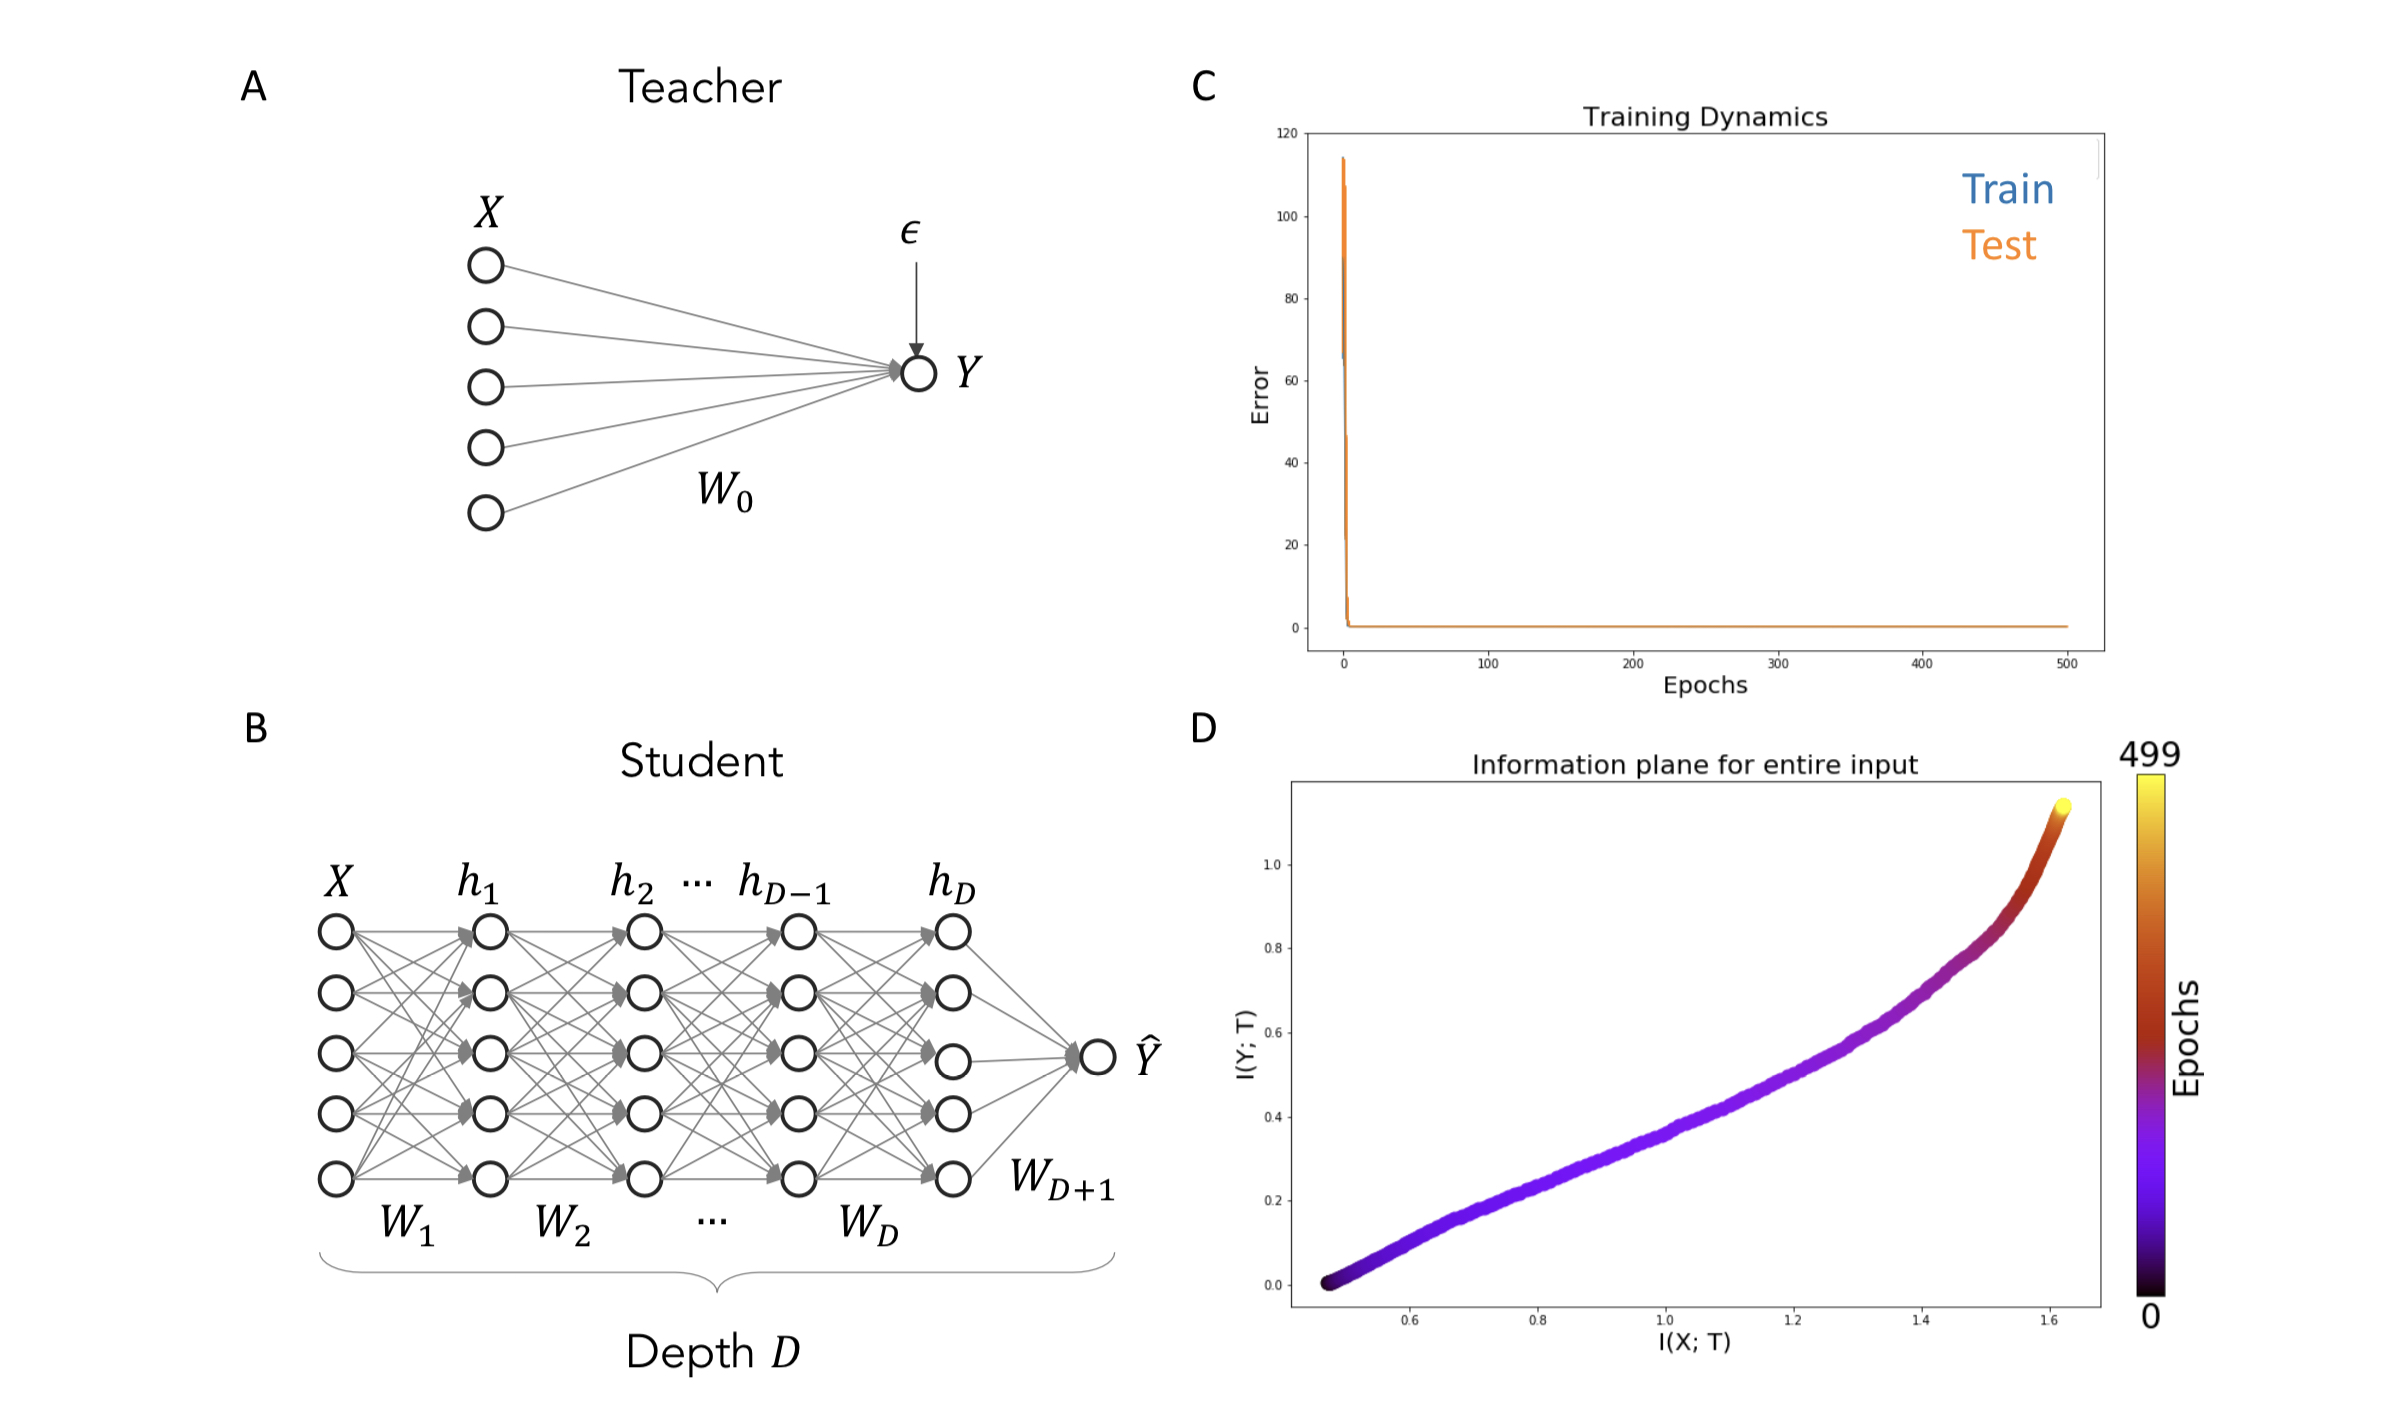
\includegraphics[width=1\textwidth, trim={0 0 0 0cm},clip]{images/InfB3.jpg}
\end{frame}

\begin{frame}{Experiments. Overtraining}
\begin{figure}[h!]
    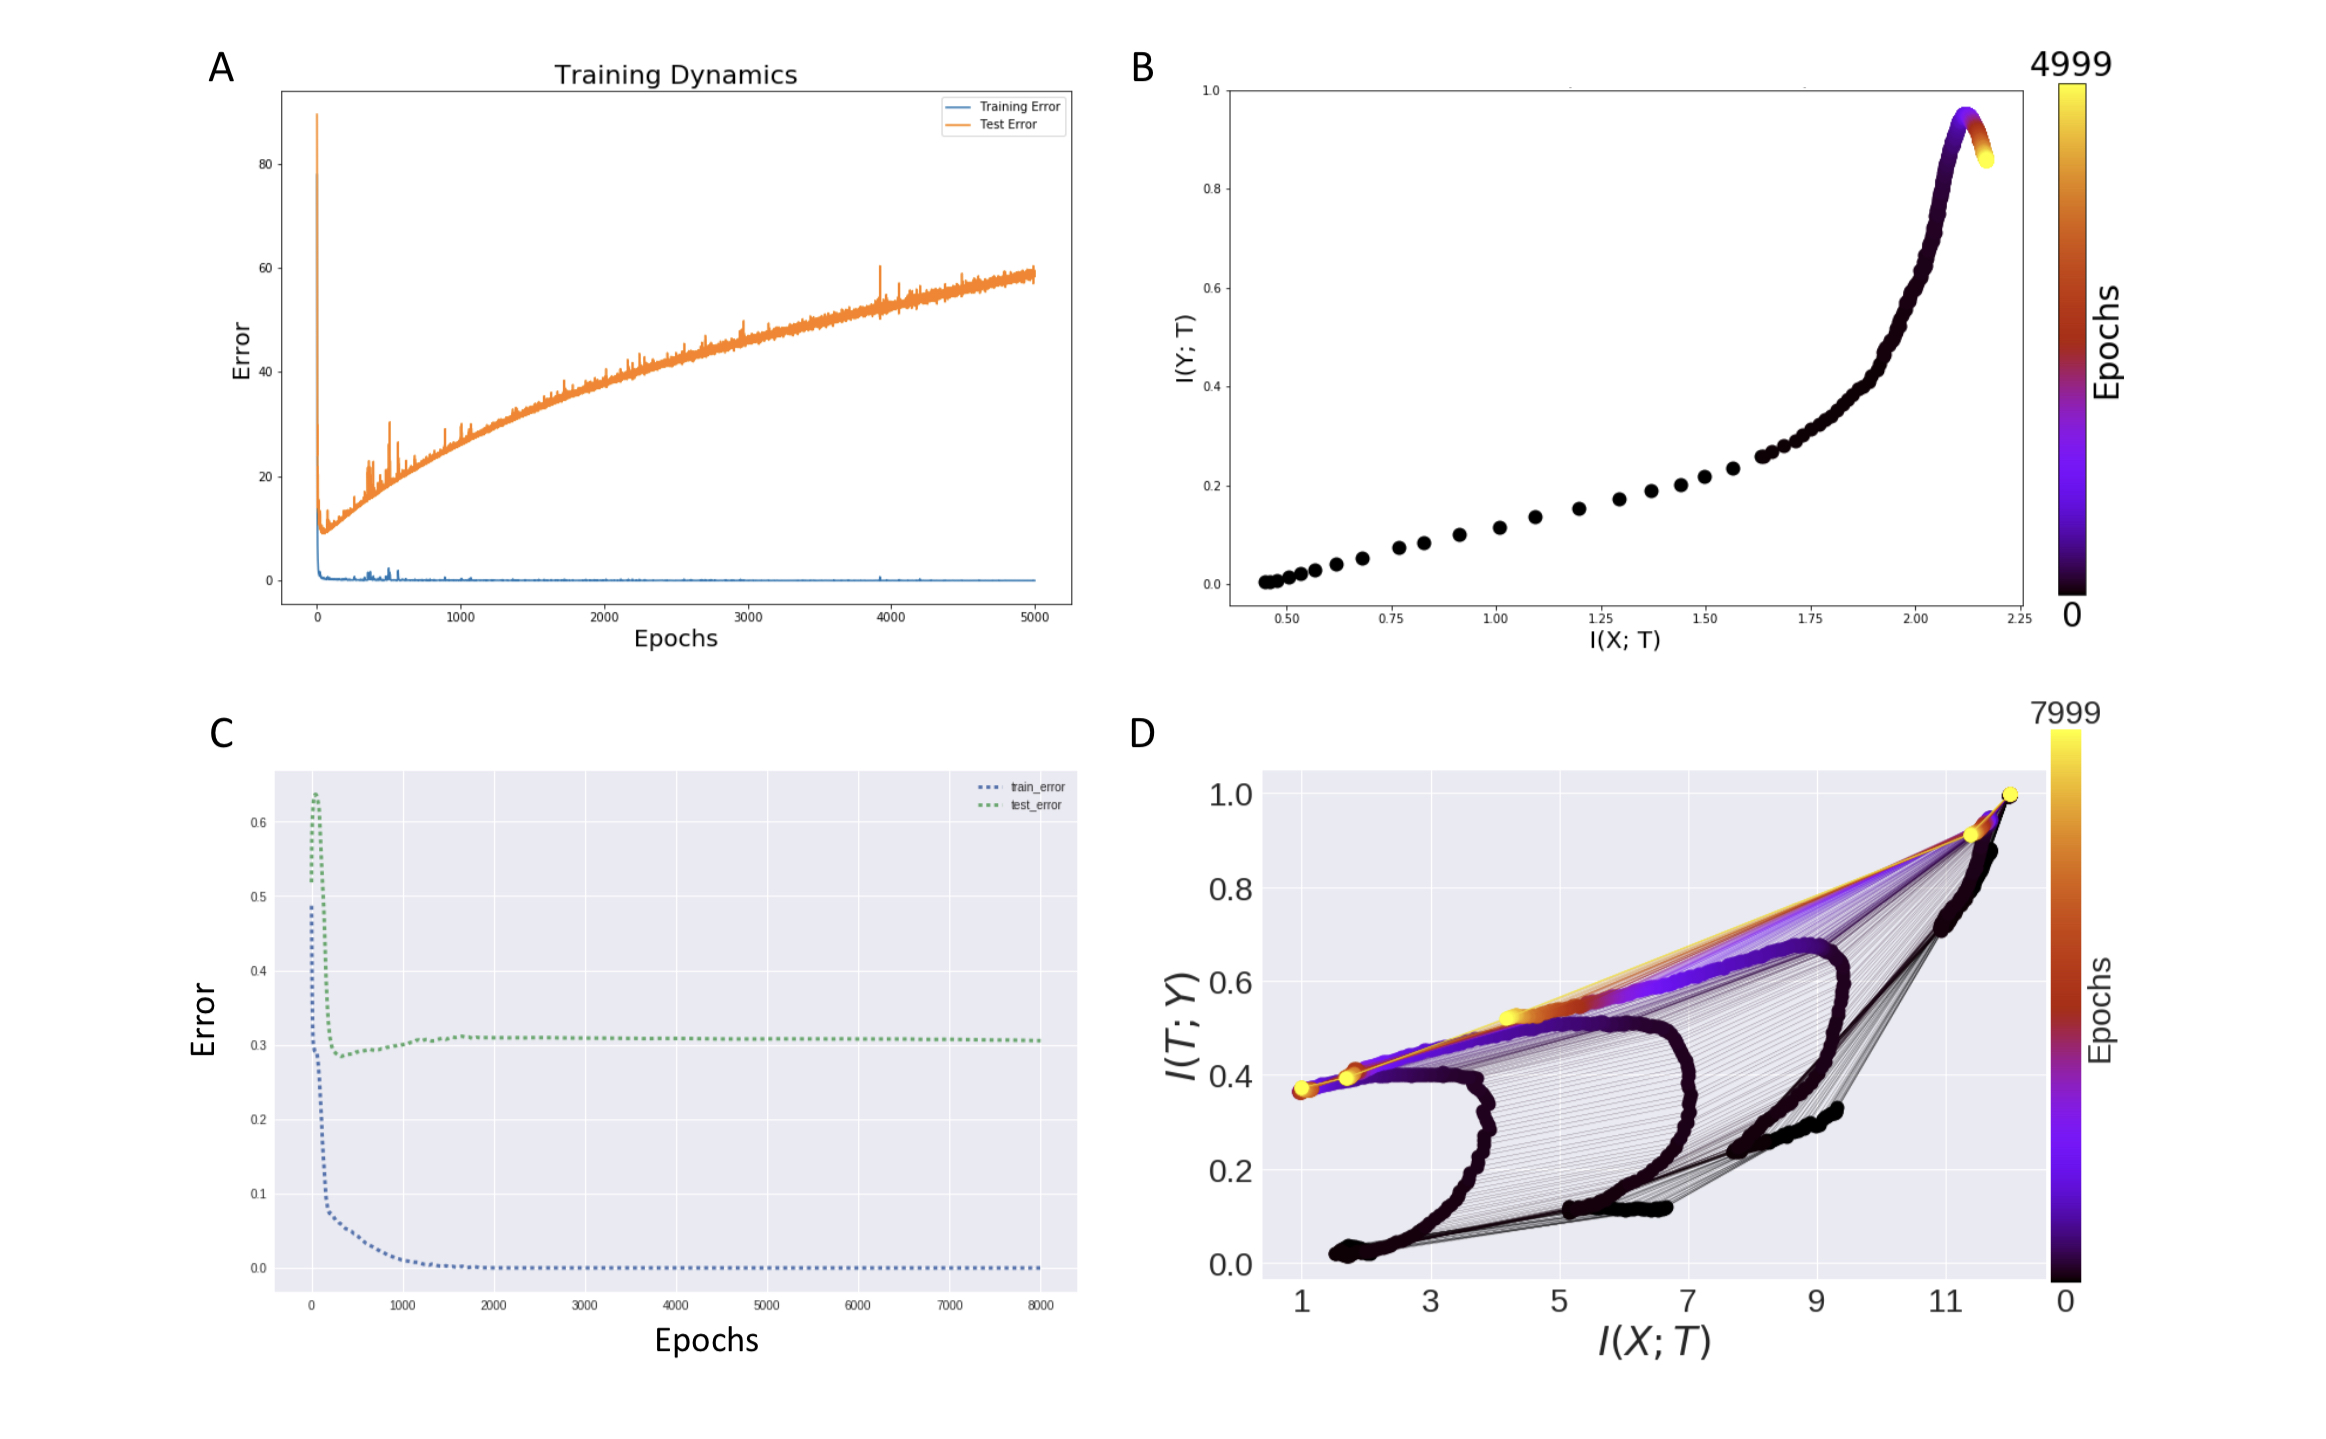
\includegraphics[width=0.9\textwidth, trim={0 0 0 0cm},clip]{images/InfB4.jpg}
    \caption{(A), (B) Overtitting with ReLU. (C), (D) Overfitting with Tanh.}
\end{figure}
\end{frame}

\begin{frame}{Experiments. Stochastic training}
\begin{figure}[h!]
    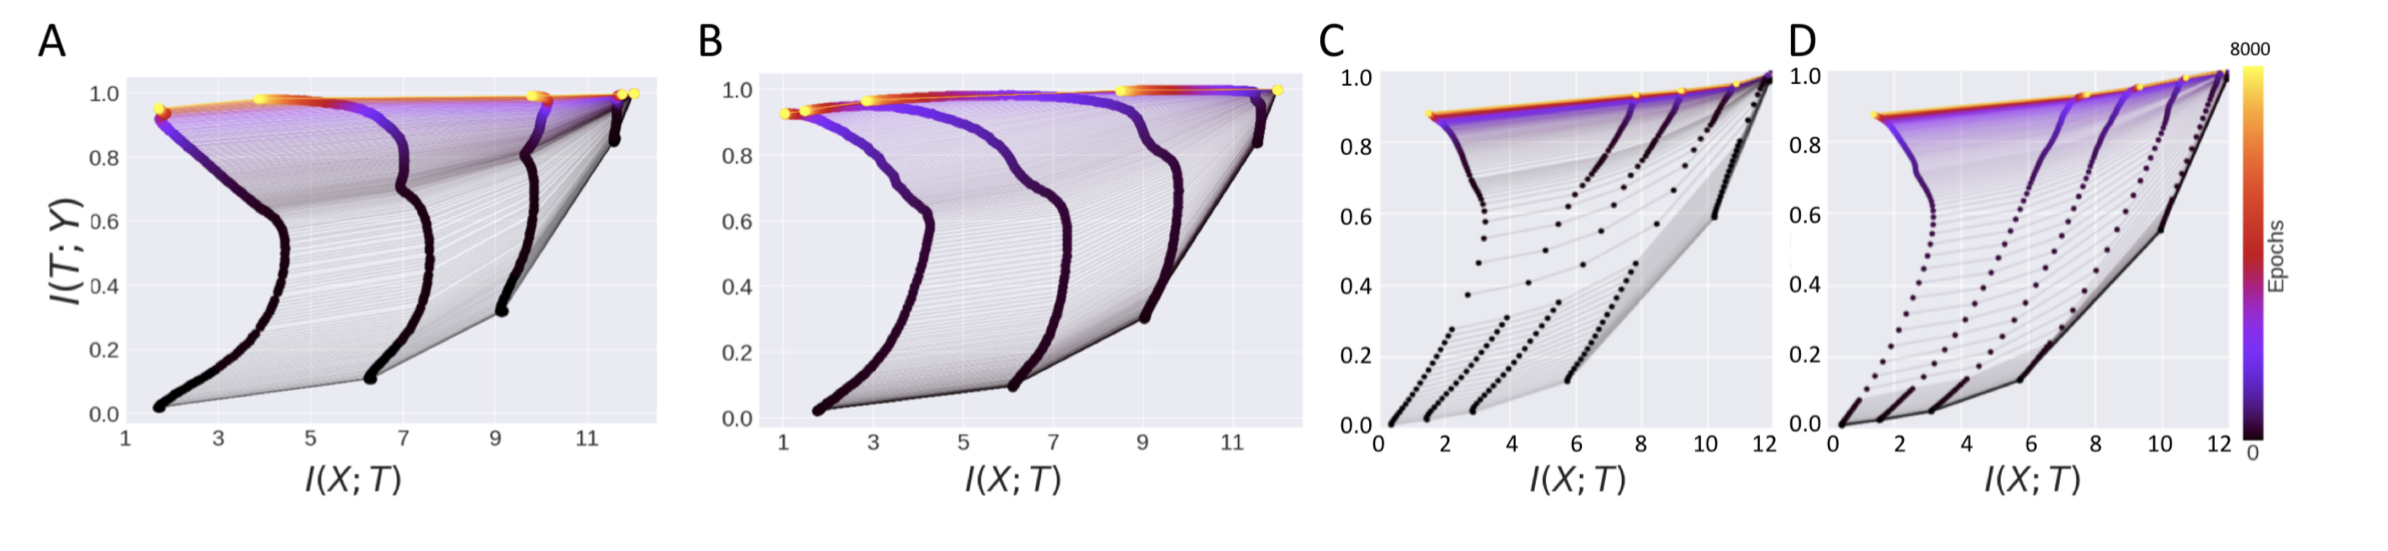
\includegraphics[width=1\textwidth, trim={0 0 0 0cm},clip]{images/InfB5.jpg}
    \caption{(A) tanh network trained with SGD. (B) tanh
network trained with BGD. (C) ReLU network trained with SGD. (D) ReLU network trained with
BGD. Both random and non-random training procedures show similar information plane dynamics.}
\end{figure}
\end{frame}

\begin{frame}{Experiments. Simultaneous fitting and compression}
\begin{figure}[h!]
    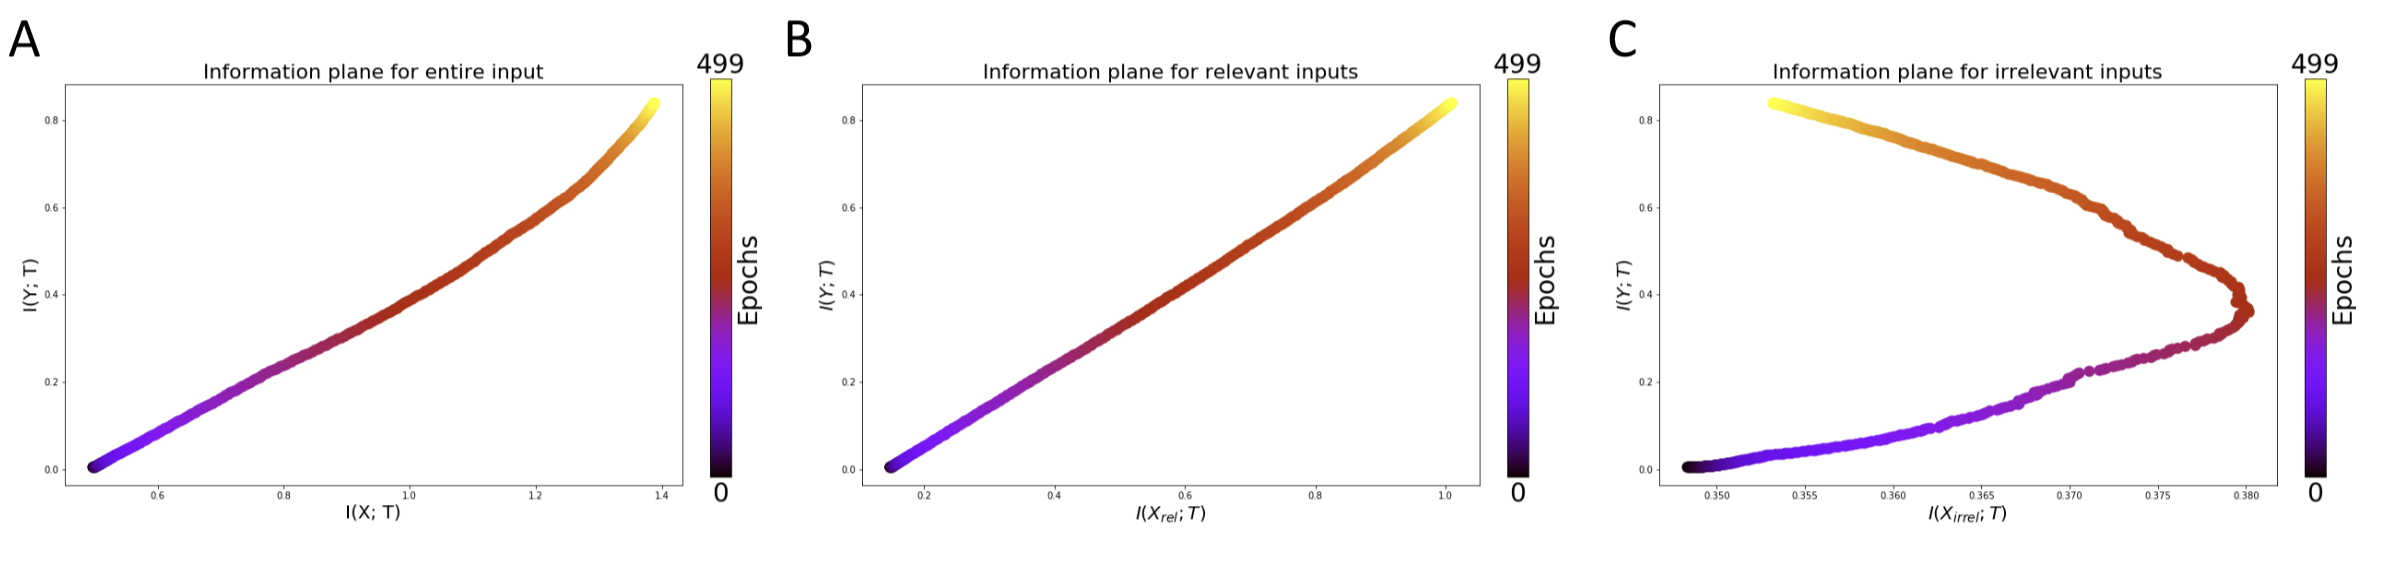
\includegraphics[width=1\textwidth, trim={0 0 0 0cm},clip]{images/InfB6.jpg}
    \caption{(A) For a task with a large task-irrelevant subspace
in the input, a linear network shows no overall compression of information about the input. (B)
The information with the task-relevant subspace increases robustly over training. (C) However, the
information specifically about the task-irrelevant subspace does compress after initially growing as
the network is trained.}
\end{figure}
\end{frame}

\begin{frame}{Literature}
\nocite{michael2018on}
\printbibliography
\end{frame}

\begin{frame}{Questions}
\textbf{1.} What is the main factor that influence the information plane trajectory of a model?

\textbf{2.} The softsign activation function is defined by $f(x) = \dfrac{x}{1 + |x|}$. Does it yield a compression phase or not? Does it cause more compression than tanh / relu? Explain why

\end{frame}

\end{document}